\chapter[Metas Decorrentes da Experiência do Usuário]{Metas Decorrentes da Experiência do Usuário}
	\label{sec:metasExperienciaUsuario}

	O objetivo de desenvolver produtos interativos agradáveis, divertidos, esteticamente apreciáveis, etc. está principalmente na experiência que estes proporcionarão ao usuário, isto é, como o usuário se sentirá na interação com o sistema. Isso envolve explicar a natureza da experiência do usuário em termos subjetivos. Assim, as metas decorrentes da experiência do usuário diferem das metas de usabilidade, que são mais objetivas, no sentido de que estão preocupadas com a maneira como os usuários lidam com um produto interativo. A relação entre os dois é mostrada na figura 1. 

	Os aspectos descritos como contribuintes para a satisfação do usuário incluem o seguinte: atenção, ritmo, jogo, interatividade, controle consciente e inconsciente, envolvimento e estilo de narrativa.

	\begin{figure}[h]
		\centering
		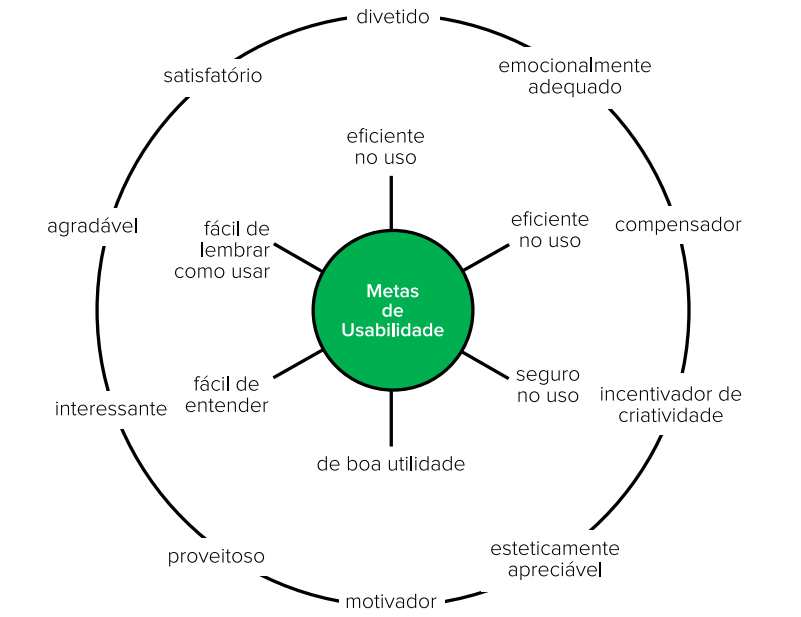
\includegraphics[scale=0.6]{metas_Experiencia_Usuario}
		\caption[Metas Decorrentes da Experiência do Usuário]{Metas Decorrentes da Experiência do Usuário. \cite{designEInteracao}}
		\label{fig:metas_Experiencia_Usuario}
	\end{figure}